\documentclass{article}
\usepackage{graphicx}
\usepackage{hyperref}
\usepackage{subcaption}
\usepackage[margin=0.5in]{geometry}
\title{CSE256: Statistical NLP Assignment 4}
\author{Pranav Verma}

\begin{document}
\maketitle
\section{IBM model 1}
	\subsection{Description of IBM model 1}
		IBM model 1 was designed as an extension of the noisy channel model for translation. A noisy channel model has two components: $p(e)$, the language model, which models the source language; and $p(f \vline e)$, the translation model. The IBM model 1 models the translation aspect of the noisy channel model. It models $p(f_{1}... f_{m} \vline e_{1}...e_{l})$, by finding the best possible alignments for each word in the foreign language sentence, $f_{i}^{(k)}$. It gets $p(f_{1},..., f_{m} \vline e_{1}, ..., e_{l})$ by computing the maximum likelihood estimates of probabilities $t(f_{i}\vline e_{j})$, which is then used to find alignments $a_{1},...,a_{m}$ which maximize the probability $p(f_{1},..., f_{m}, a_1,..., a_m \vline e_{1}, ..., e_{l})$.
		\\IBM Model 1 has some severe limitations, chief of which is that each word in the source sentence can only translate to one word in the target sentence. This is not the case in real world, and thus this model is severely limited. Also, the position of the target word in target language is independent of the location of source word in the source sentence, and also independent of the positions of other words in the sentences. It does not consider the fact that for some translations, words which appear after the other in the source translations will also appear after each other in the target sentence. It will treat this language pair translation the same as it would treat language pairs in which the words appear in reverse order in the target sentence.
	\subsection{Description of EM algorithm}
		The Expectation Maximization (EM) algorithm is used to find out the maximum likelihood estimates of the unobserved data ($t(f_{i}\vline e_{j})$) using an iterative procedure. In the expectation step, it calculates the likelihood of finding $i^{th}$ foreign language word and $j^{th}$ language word together using the current estimates of $t(f_{i}\vline e_{j})$ over the whole model, and then uses these estimates to compute the parameter $t(f_{i}\vline e_{j})$ which would maximize the maximum likelihood value computed in the E step.
		\\ The EM algorithm is a good way to estimate the latent variables values. However, there is a possibility that the parameters found are not the globally optimum parameters (i.e. better values of these parameters may exist). The performance is dependent on the starting point of the algorithm, and is therefore not guarenteed to yield the best results.
	\subsection{Method Overview}
		To implement IBM model 1, we stored the values $t(f \vline e)$ in a dictionary, for each English word $e$ and Spanish word $f$ in the corresponding sentences in the English and Spanish corpora. Similarly, the values $c(e,f), c(e), c(j \vline i,l_{k},m_{k}), c(i,l_{k},m_{k})$ were all stored in dictionaries, with tuples of $e,f,i,j,l_{k},m_{k}$ as keys. This allowed us to store the parameters as sparsely as possible, saving a lot of memory. 
		\\$t(f \vline e)$ was initialised with $\frac{1}{n(e)+1}$ where $n(e)$ was the frequency count of the word $e$ in the English corpus.
		\\Then, the EM algorithm was a straight-forward procedure, where we started by setting $c=0$ for all keys. Then we incremented the counts of the $c$ dictionaries by $\delta(k,i,j)$, which was calculated using our current estimates of $t(f \vline e)$, for all $e$,$f$ in all the sentence pairs in the English and Spanish corpora. Then, using these counts $c$, we updated the values of $t(f \vline e)$ for all English words $e$ and Spanish words $f$ in the sentence pairs of the respective corpora. Repeating the above procedure 5 times yielded a good approximation of the value $t(f \vline e)$
		\\To get the alignments for $i^{th}$ Spanish word $f_{i}^{k}$ in $k^{th}$ sentence, we simply found the location of $j^{th}$ English word $e_{j}^{k}$ in the corresponding $k^{th}$ English sentence which yielded the maximum value of $t(f \vline e)$. The alignment was finally represented as $\left[k\quad j\quad i\right]$.
	\subsection{Results}
		By performing 5 iteration of the EM algorithm for the IBM model 1, as described above, we get the following values:
		\begin{table}[htbp]
			\center
			\begin{tabular}{|c|c|c|c|c|}
				\hline
				Type&Total&Precision&Recall&F1-Score\\
				\hline
				total&        5920&     0.412&        0.426&        0.419\\
				\hline
			\end{tabular}
			\caption{Performance of IBM model 1 on dev data}
		\end{table}
	\subsection{Discussion}
	As a function of iterations, we see that the model iteratively learns optimal alignments. This is reflected in the increasing F1 scores:

	\begin{table}[htbp]
		\center
		\begin{tabular}{|c|c|c|c|c|c|}
			\hline
			Iteration&Type&Total&Precision&Recall&F1-Score\\
			\hline
			1&total&5920&    0.222 &       0.230 &       0.226\\
			\hline
			2&total&        5920&     0.369&        0.381&        0.375\\
			\hline
			3&total&        5920&    0.401&        0.414&        0.407\\
			\hline
			4&total&        5920&     0.408&        0.422&        0.415\\
			\hline
			5&total&        5920&     0.412&        0.426&        0.419\\
			\hline
		\end{tabular}
		\caption{Performance of IBM model 1 on dev data as a function of number of iterations of the EM algorithm}
	\end{table}
\section{IBM model 2}

	\subsection{Description of IBM model 2}
		IBM model 2 was designed to be an improvement over model 1. It models the $p(f\vline e)$ using two parameters, $q(j\vline i,l,m)$ and $t(f\vline e)$. The first parameter describes the likelihood that the $j^{th}$ word in source sentence of length $l$ aligns to the $i^{th}$ word in the target sentence of length $m$. This will allow us, for example, to capture the tendency for words close to the beginning of the foreign sentence to be translations of words close to the beginning of the source language sentence. 
		\\However, there's one key limitation in translation that even IBM model 2 fails to address: the source word can translate to zero or one or more than one words in the foreign language. It does not model these tendencies in its translation model at all.

	\subsection{Method Overview}
		The IBM model 2 was very similar to the IBM model 1 described above. We started with $t(f \vline e)$ as estimated from 5 iterations of EM algorithm in IBM model 1. We also kept track of another parameter $q(j \vline i,l_{k},m_{k})$, using a dictionary, with the tuple $(i,j,l_{k},m_{k})$ as keys for the dictionary. We initialized it using $q(j \vline i,l_{k},m_{k})=\frac{1}{l_{k}+1}$, where $l_{k}$ was the length of $k^{th}$ English sentence.
		\\Then, as we did in the case of IBM model 1, we initialized $c=0$ for all keys, and for all words in each sentence in the corpora, updated it using 
		$$\delta(k,i,j) = \frac{q(j \vline i,l_{k},m_{k})t(f_{i}^{(k)} \vline e_{j}^{(k)})}{\Sigma_{k=0}^{l_{k}} q(j \vline i,l_{k},m_{k})t(f_{i}^{(k)} \vline e_{j}^{(k)})} $$
		using the current estimates of $t(f_{i}^{(k)} \vline e_{j}^{(k)})$ and $q(j \vline i,l_{k},m_{k})$ for each Englis word $e_{j}^{k}$, and spanish word $f_{i}^{k}$ in $k^{th}$ sentence pairs in the corpora. 
		\\Using these updated estimates of $c$, we updated our estimates of $q$ and $t$, using:
		$$q(j \vline i,l,m) = \frac{c(j \vline i,l,m)}{c(i,l,m)} $$
		and $$t(f \vline e) = \frac{c(e,f)}{c(e)} $$
		5 iterations of this EM algorithm were run to get estimates of $t$ and $q$. Using these estimates, we predicted the alignments for $i^{th}$ in $k^{th}$ sentence by finding the $j^{th}$ word such that the value of $q(j \vline i,l,m)t(f_{i} \vline e_{j})$ was maximum. The alignment was then recorded as the tuple $\left[k\quad j\quad i\right]$
	\subsection{Results}
		Using the algorithm described above, and running for five iterations, we get the following results:
		\begin{table}[htbp]
			\center
			\begin{tabular}{|c|c|c|c|c|}
				\hline
				Type&Total&Precision&Recall&F1-Score\\
				\hline
				total&        5920&     0.442&        0.456&        0.449\\
				\hline
			\end{tabular}
			\caption{Performance of IBM model 2 on the dev data set after 5 iterations of EM algorithm}
		\end{table}
		We note that the final F1 score after 5 iterations was $0.449$, a clear improvement over IBM model 1.

	\subsection{Discussion}
		We present below the performance of our model at the end of each iteration. We see that the model generally performs better each iteration, as it updates the $t$ and $q$ parameters iteratively on the whole dataset.
		\begin{table}[htbp]
			\center
			\begin{tabular}{|c|c|c|c|c|c|}
				\hline
				Iteration&Type&Total&Precision&Recall&F1-Score\\
				\hline
				1&total&        5920&     0.431&        0.445&        0.438\\
				\hline
				2&total&        5920&     0.436&        0.451&        0.443\\
				\hline
				3&total&        5920&     0.439&        0.454&        0.446\\
				\hline
				4&total&        5920&     0.438&        0.453&        0.445\\
				\hline
				5&total&        5920&     0.442&        0.456&        0.449\\
				\hline
			\end{tabular}
			\caption{Performance of IBM model 2 on the dev data set as a function of number of iterations of EM algorithm run}
		\end{table}
	\subsubsection{Aligned and Misaligned sentences}
		We present the alignment matrices for aligned and misaligned cases. Green cells highlight alignments predicted by both the gold standard and our model. Gold cells represent alignments from the gold standard missed by our model, and red cells represent incorrect alignments predicted by our model.
		\begin{figure}[htbp]
			\center
			\begin{subfigure}{\textwidth}
				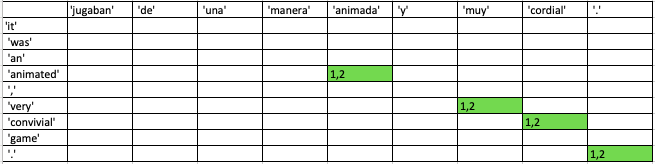
\includegraphics[width=0.7\textwidth]{alignment.png}
				\subcaption{Sentence 1}
			\end{subfigure}
			\begin{subfigure}{\textwidth}
				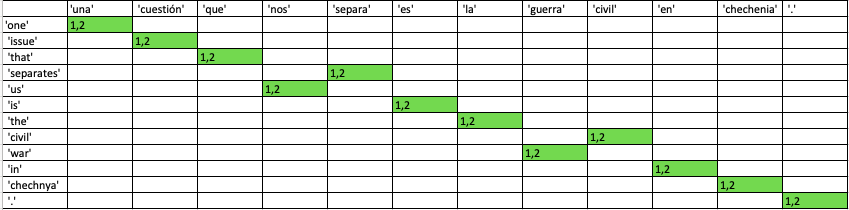
\includegraphics[width=0.7\textwidth]{alignment_1.png}
				\subcaption{Sentence 2}
			\end{subfigure}
			\caption{Correctly Aligned sentences}
		\end{figure}

		\begin{figure}[htbp]
			\center
			\begin{subfigure}{\textwidth}
				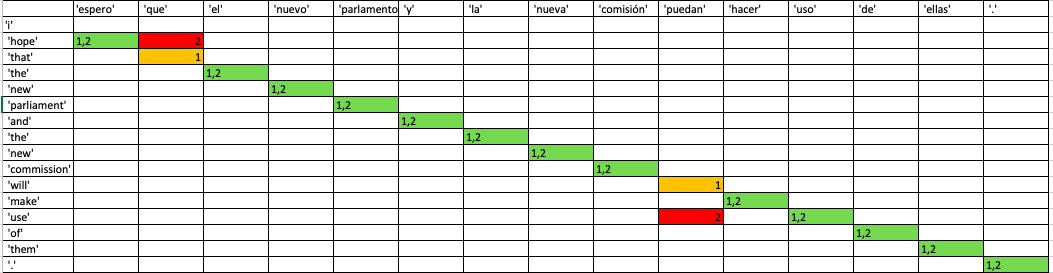
\includegraphics[width=0.7\textwidth]{misalignment.png}
				\caption{Sentence 1}
			\end{subfigure}
			\begin{subfigure}{\textwidth}
				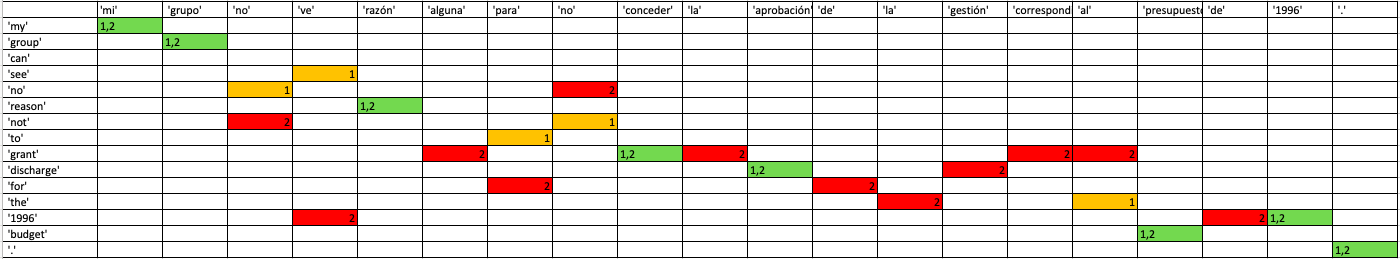
\includegraphics[width=0.7\textwidth]{misalignment_1.png}
				\subcaption{Sentence 2}
			\end{subfigure}
			\caption{Incorrectly Aligned sentences}
		\end{figure}


\section{Growing Alignments}

	\subsection{Method Overview}
		We started with the alignments which we got from the IBM model 2 described above. Then we found the alignments by going in the reverse direction: English to foreign. Then, we took the alignments which were predicted by both these methods (calling these the intersection of the two alignment sets), and all the alignments by any of these two methods (calling these the union of the two alignment sets). We start from the intersection set, and iteratively add the alignments from the union set which are not in the intersection set. We do this by generating the alignment matrix for each sentence. We put alignments in the intersection as 1, and alignments in union as -1.
		\\Our heuristic is to add neighbouring alignments, i.e. if $(i,j)$ is not currently in the alignments, but one of its neighbours are, then we add $(i,j)$ into the alignment set. In the alignment matrix, it is equivalent to turing all -1's which have 1 as their immediate neighbours into +1's, and adding those alignments to the intersection set.
		\\We do this procedure over all sentences, and repeat the whole process till we have no more alignments to add this way. We present our results below.
	\subsection{Results}
		The intersection alignment set had the following scores:
		\begin{table}[htbp]
			\center
			\begin{tabular}{|c|c|c|c|c|}
				\hline
				Type&Total&Precision&Recall&F1-Score\\
				\hline
				total&        5920&     0.775&        0.352&        0.485\\
				\hline
			\end{tabular}
			\caption{Performance of Intersection alignments}
		\end{table}

		The union alignment set had the following scores:
		\begin{table}[htbp]
			\center
			\begin{tabular}{|c|c|c|c|c|}
				\hline
				Type&Total&Precision&Recall&F1-Score\\
				\hline
				total&5920&0.363&0.565&0.442\\
				\hline
			\end{tabular}
			\caption{Performance of Union alignments}
		\end{table}
		\\We note that intersection alignment set has a high precision score, while union set has a high recall score. Combining the alignments from these two allow us to get alignments which balance the precision and recall, and achieve an overall higher F1 score than both:
		\begin{table}[htbp]
			\center
			\begin{tabular}{|c|c|c|c|c|c|}
				\hline
				Iteration&Type&Total&Precision&Recall&F1-Score\\
				\hline
				1&total&        5920&     0.673&        0.453&        0.541\\
				\hline
				2&total&        5920&     0.662&        0.464&        0.545\\
				\hline
				3&total&        5920&     0.659&        0.466&        0.546\\
				\hline
				4&total&        5920&     0.658&        0.467&        0.547\\
				\hline
				5&total&        5920&     0.658&        0.468&        0.547\\
				\hline
				6&total&        5920&     0.658&        0.468&        0.547\\

				% 1&total&        5920&     0.700&        0.415&        0.521\\
				% \hline
				% 2&total&        5920&     0.690&        0.423&        0.524\\
				% \hline
				% 3&total&        5920&     0.687&        0.425&        0.525\\
				% \hline
				% 4&total&        5920&     0.687&        0.425&        0.525\\
				% \hline
				% 5&total&        5920&     0.687&        0.426&        0.526\\
				% \hline
				% 6&total&        5920&     0.687&        0.426&        0.526\\
				\hline
			\end{tabular}
			\caption{Growing Alignments: Performance as we add more neigbouring alignments from union of alignments to intersection, over multiple iterations}
		\end{table}
		\\We note that as we add more and more of alignments, we are able to achieve a better F1 score.

	\subsection{Another heuristic towards growing alignments}
	We tried another heuristic to grow the alignments, similar to the one described in section 4.5 of \href{https://www.aclweb.org/anthology/N03-1017.pdf}{https://www.aclweb.org/anthology/N03-1017.pdf}. For each sentence, we built the alignment matrix, and we looked at words which were unaligned in the intersection set, and added alignments from the union set if they existed. We did this for each sentence in the sentence pairs of the corpus. After one complete pass over the entire corpus, we evaluated the model's performance:
	\begin{table}[htbp]
	\center
	\begin{tabular}{|c|c|c|c|c|}
	\hline
	Type&Total&Precision&Recall&F1-Score\\
	\hline
	total&        5920&     0.558&        0.440&        0.492\\
	\hline
	\end{tabular}
	\caption{Performance using the new heuristic, after one complete pass over the entire corpus}
	\end{table}
	\\We see that our model performs better than IBM model 2, and improves over the intersection alignment set.
\end{document}